%%% LaTeX Template: Two column article
%%%
%%% Source: http://www.howtotex.com/
%%% Feel free to distribute this template, but please keep to referal to http://www.howtotex.com/ here.
%%% Date: February 2011

%%% Preamble
\documentclass[	DIV=calc,%
							paper=a4,%
							fontsize=12pt,%
							onecolumn]{scrartcl}	 					% KOMA-article class

\usepackage{lipsum}													% Package to create dummy text
\usepackage[english]{babel}										% English language/hyphenation
\usepackage[protrusion=true,expansion=true]{microtype}				% Better typography
\usepackage{amsmath,amsfonts,amsthm}					% Math packages
\usepackage[pdftex]{graphicx}									% Enable pdflatex
\usepackage[svgnames]{xcolor}									% Enabling colors by their 'svgnames'
\usepackage[hang, small,labelfont=bf,up,textfont=it,up]{caption}	% Custom captions under/above floats
\usepackage{epstopdf}												% Converts .eps to .pdf
\usepackage{subfig}													% Subfigures
\usepackage{booktabs}												% Nicer tables
\usepackage{fix-cm}													% Custom fontsizes
\usepackage[utf8]{inputenc}
\usepackage[top=2.5cm, bottom=2.5cm, left=2.5cm, right=2.5cm]{geometry}
\usepackage[ddmmyyyy]{datetime}
\usepackage{verbatim}
\addto\captionsenglish{%
	\renewcommand\tablename{Tabela}
	\renewcommand\figurename{Figura}
} 
 

 
%%% Custom sectioning (sectsty package)
\usepackage{sectsty}													% Custom sectioning (see below)
\allsectionsfont{%															% Change font of al section commands
	\usefont{OT1}{phv}{b}{n}%										% bch-b-n: CharterBT-Bold font
	}

\sectionfont{%																% Change font of \section command
	\usefont{OT1}{phv}{b}{n}%										% bch-b-n: CharterBT-Bold font
	}



%%% Headers and footers
\usepackage{fancyhdr}												% Needed to define custom headers/footers
	\pagestyle{fancy}														% Enabling the custom headers/footers
\usepackage{lastpage}	

% Header (empty)
\lhead{}
\chead{}
\rhead{}
% Footer (you may change this to your own needs)

%% ====================================
%% ====================================
%% mude o rodape  do projeto
%% ====================================
%% ====================================

\lfoot{\footnotesize \texttt{Cabeamento Estruturado - Redes VI} \textbullet ~Certificação}


\cfoot{}
\rfoot{\footnotesize página \thepage\ de \pageref{LastPage}}	% "Page 1 of 2"
\renewcommand{\headrulewidth}{0.0pt}
\renewcommand{\footrulewidth}{0.4pt}



%%% Creating an initial of the very first character of the content
\usepackage{lettrine}
\newcommand{\initial}[1]{%
     \lettrine[lines=3,lhang=0.3,nindent=0em]{
     				\color{DarkGoldenrod}
     				{\textsf{#1}}}{}}



%%% Title, author and date metadata
\usepackage{titling}															% For custom titles

\newcommand{\HorRule}{\color{DarkGoldenrod}%			% Creating a horizontal rule
									  	\rule{\linewidth}{1pt}%
										}

\pretitle{\vspace{-25pt} \begin{flushleft} \HorRule 
				\fontsize{50}{50} \usefont{OT1}{phv}{b}{n} \color{DarkRed} \selectfont 
				}

%% ====================================
%% ====================================
%% mude o titulo  do projeto
%% ====================================
%% ====================================

\title{Projeto de Cabeamento Estruturado para Edifício de dois Andares}					% Title of your article goes here

%% ====================================



\posttitle{\par\end{flushleft}\vskip 0.5em}

\preauthor{\begin{flushleft}
					\large \lineskip 0.5em \usefont{OT1}{phv}{b}{sl} \color{DarkRed}}
\author{Augusto Fernando Ruis, Clayton Camargo Oliveira, João Emiliano dos Santos, Renan Ribeiro Sakomoto Zuculin}  	% Author name goes here


\postauthor{\footnotesize \usefont{OT1}{phv}{m}{sl} \color{Black} 
					\\Universidade Tecnológica Federal do Paraná - Câmpus Cornélio Procópio 								% Institution of author
					\par\end{flushleft}\HorRule}

\date{}																				% No date




%%% Begin document
\begin{document}
\maketitle
\thispagestyle{fancy} 	
\thispagestyle{empty}		% Enabling the custom headers/footers for the first page 
% The first character should be within \initial{}




%% ====================================
%% ====================================
%% mude o resumo  do projeto
%% ====================================
%% ====================================
\initial\textbf{Esta documentação tem como objetivo demonstrar na prática a elaboração de um projeto de cabeamento estruturado, embasando-se em normas nacionais e internacionais como, por exemplo, NBR-14565-2007 e TIA/EIA-568-B. A implantação do presente projeto será realizado de forma fictícia em um edifício comercial de dois andares, onde o piso um possui 6 salas e o piso 2 possui 10 salas com tomadas de telecomunicações.
A rede de cabeamento estruturado será criada do zero com o intuito de administrar de uma forma precisa e eficaz os recursos de dados e voz, atendendo as necessidades momentâneas e futuras de uma organização.
Os elementos de rede presente nos pisos serão devidamente identificados utilizando-se de padrões, o layout se dá por meio de um cabeamento horizontal que interliga cada área de trabalho aos armários de telecomunicações presentes nos dois pisos e esses por sua vez são interligados por um backbone.}

%% ====================================
%%\begin{figure}
%%	\centering
%%	\includegraphics{utfpr}
%%\end{figure}

\vspace{2cm}
\centerline{\textit{\textbf{\today}}}

\clearpage
    \renewcommand*\listfigurename{Lista de figuras}
\listoffigures

\renewcommand*\listtablename{Lista de tabelas}
\listoftables




\clearpage
\renewcommand{\contentsname}{Sumário}
\tableofcontents
\clearpage

%% ====================================
%% ====================================
%% Inicio do texto
%% ====================================
%% ====================================
\section{Introdução}
O projeto tem a finalidade de atender a necessidade de interligação de dois andares, sendo o piso 1 com 6 salas e o piso 2 com 10 salas, levando pontos de redes com acesso a dados e voz para cada área de trabalho do edifício. 
Atualmente o prédio não conta com nenhum equipamento de TI facilitando a implantação do projeto em questão.
Basicamente o projeto utilizará um armário de telecomunicação em cada piso interligados por um backbone e em cada armário de telecomunicação teremos um path panel e switch para dados e um path panel e switch para voz.


\subsection{Benefícios}
Com a implantação de um projeto de cabeamento estruturado seguindo normas como NBR-14565-2007 e TIA/EIA-568-B os principais benefícios são que a probabilidade de ocorrer erros na camada física diminui muito, por conta dos equipamentos e testes realizados no processo, a identificação de problemas posteriores na camada física podem ser identificados de forma mais fácil por conta da identificação dos pontos de redes e com a estruturação a rede pode ser facilmente expandida.


\section{Usuários e Aplicativos}

A estrutura a ser aplicada poderá atender até 64 usuários simultaneamente, número definido pela quantidade de pontos de rede a serem instalados, sendo que a estrutura final contará com a possibilidade de ampliação da rede como um todo, visto que a empresa possui metas de crescimento. O número de usuários e aplicativos utilizados serão especificados a seguir.


%%Galera aqui preciso de ajuda para demonstrar como podemos expandir essa rede colocando mais equipamentos no rack ou nos pontos de rede, e %%estipular uma quantidade inicial de usuários que a rede atende. Não precisamos detalhar muito quais equipamentos e quantidade pois essas %%informações devemos colocar no plano de expansão em um próximo tópico. Aguardo sugestões.

%%11/08/2016 - Augusto Ruis: 
%%GALERA, FIZ A CONTA DE 16 SALAS X 4 PONTOS DE REDE CADA SALA:
 

\subsection{Usuários}
Definindo o tópico de cima partimos para esse.


\subsection{Aplicativos}
Aqui podemos bolar algo tipo uma estrutura comercial com as aplicações necessárias para toca a empresa?


\section{Estrutura predial existente}

O prédio que o cabeamento irá atender é composto por piso 1 que possui 6 salas com tomadas de telecomunicação e o piso 2 que é composto por 10 salas com tomadas de telecomunicação. OBS: Vou abrir a planta no Autocad e mando a imagem para a gente melhorar esse tópico.   

Deve conter uma descrição geral, indicando a possível distância entre os pontos de rede e restrições de instalação.


\section{Planta Lógica - Elementos estruturados}


\subsection{Topologia}
Proposta futura, proposta após implantação.
Deve conter o diagrama da rede. Atente-se a redundância  e ligações truncadas.
Deve explicar todos termos e componentes utilizados nestas plantas. Por exemplo: entrance facility, work area, horizontal cabling, etc..

Todos os elementos das figuras devem ser explicados. 
Crie esboço da configuração dos racks e brackets. Explique cada um dos componentes. Você pode criar uma tabela contendo figuras dentro, ou criar uma tabela e incluí-la como imagem. Por exemplo, verifique a tabela \ref{tab1}.

%%\begin{table}[h!]
\centering
\caption{Diagrama Lógico de rede}
\label{tab1}
\begin{tabular}{|l|l|l|}
\hline
\multicolumn{1}{|l|}{Armários de Telecomunicação} \\ \hline
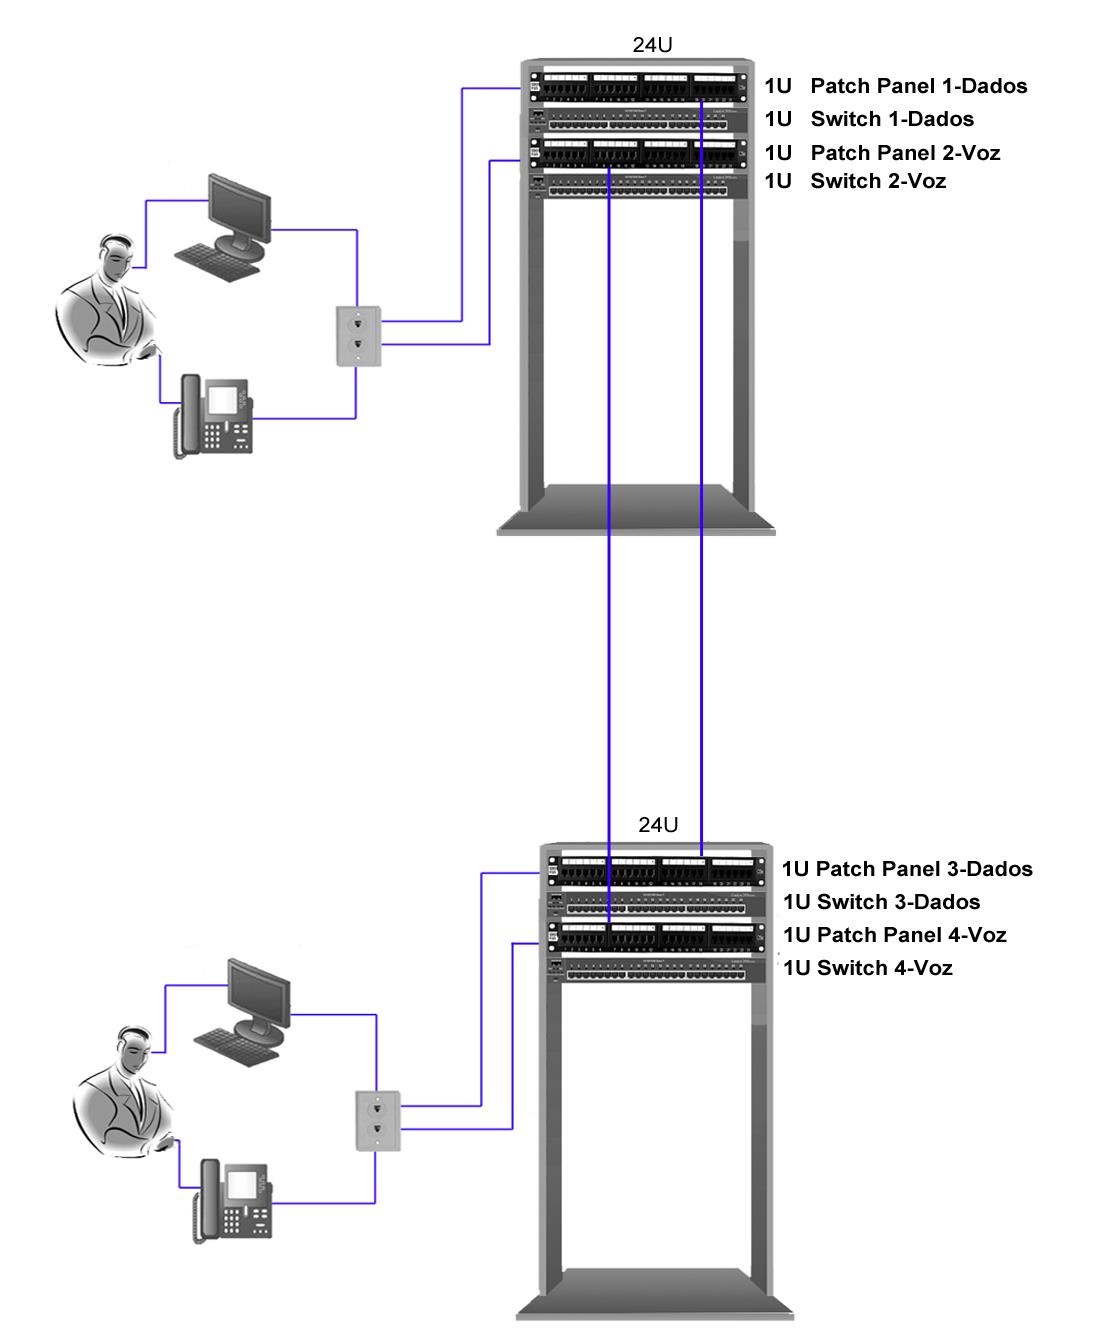
\includegraphics[scale=0.2]{fig1}        \\ \hline

\end{tabular}
\end{table}

\subsection{Encaminhamento}
Eletrodutos, calhas, e qualquer material em que os cabos serão alojados/alocados.

\subsection{Memorial descritivo}

Relacione todos os equipamentos passivos que serão utilizados, tipo, fabricante, quantidade.

\subsection{Identificação dos cabos}

\section{Implantação}
Estabeleça um cronograma de implantação:
Remoção de equipamentos existentes (destino para descarte), instalação dos condutores, instalação dos cabos, 
identificação dos cabos, montagem dos racks, certificação, etc... Crie atividades e estabeleça o tempo de execução. Se for um projeto real, indique também quais os responsáveis pela execução do projeto e de cada uma das etapas.

Defina marcas (e padrões) e fornecedores se for o caso. Atenção a contratados e subcontratados para a realização das atividades. Estabeleça a responsabilidade de execução da atividade e também da validação dela.

Utilize algum software para gerear o cronograma. Excel,etc. O fundamental é dividir em etapas, descrever e estimar o tempo de cada uma delas.

Segue uma relação de ferramentas:
http://asana.com/, 
https://trello.com/, 
http://www.ganttproject.biz/, 
http://www.orangescrum.org/. 

\section{Plano de certificação}
Quais seriam as etapas para a certificação? 
Quais os locais e horários para execução da certificação na rede? Toda rede será certificada?
Como os testes seriam executados?
Quais relatórios de certificação serão (ou deveriam ser) entregues? 

\section{Plano de manutenção}

Revisões periódicas na rede, emissão de certificados para novos pontos.

\subsection{Plano de expansão}
Existe um plano de expansão? Quantos novos pontos poderão ser acrecidos na rede, antes de migração de equipamentos na camada 2? Se houver expansão, quais equipamentos deverão ser direcionados para as estremidades da rede? 


\section{Orçamento}
Crie uma relação de orçamentos baseado na seções anteriores.

\section{Referências bibliográficas}
Utilize o mendley, o jabref ou diretamente o bibtex para gerenciar suas referências biliográficas. As referências são criadas automaticamente de acordo com o uso no texto.

Exemplo: Redes de computadores, segundo \cite{t2013} é considerada..... Já \cite{kurose2010} apresenta uma versão...

Analisando os pressupostos de \cite{ref3} e \cite{ref4} concluimos que....


\renewcommand\refname{} %%Referências bibliográficas}  
\bibliographystyle{ieeetr}
\bibliography{referencias}  

%% ***********************************************************************
%% === remover daqui =====================================================
%% ***********************************************************************

\section{Elementos textuais - Alguns exemplos}

Esta seção apresenta exemplos de elementos textuais. \textbf{Remova-a da versão final do texto}.


\subsection{Colocar elementos em itens}

Texto antes da lista

\begin{itemize}
	\item First item in a list 
	\item Second item in a list 
	\item Third item in a list
\end{itemize}

\subsubsection{Uma sub seçao de terceiro nivel}

Exemplo de uma subseção

\subsection{Tabelas}

Utilize o site http://www.tablesgenerator.com/ para elaborar as tabelas de seu trabalho.
Para adicionar uma tabela utilize: a tag input, passando o arquivo da tabela como parametro

%%\begin{table}[h!]
\centering
\caption{Legenda dos Equipamentos}
\label{tab2}
\begin{tabular}{|l|l|l|}
\hline
\multicolumn{1}{|l|}{Descrição dos Materiais} \\ \hline
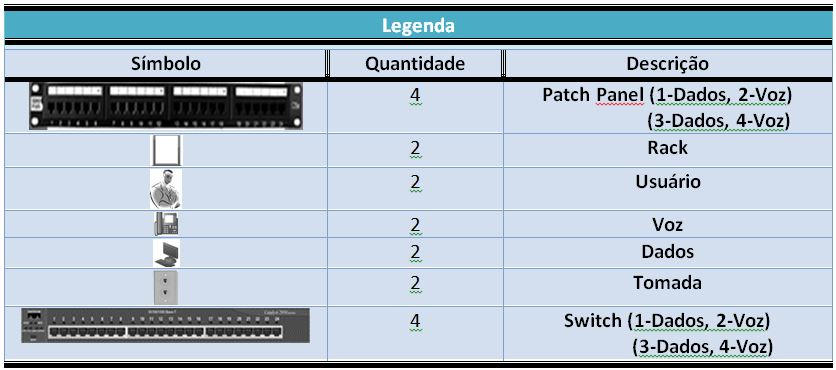
\includegraphics[scale=0.5]{fig2}        \\ \hline

\end{tabular}
\end{table}

Dentro do arquivo você deve definir o label e pode utilizá-lo para referenciar. Exemplo:
Na tab \ref{tab2} temos a relação de ....


Você também pode modificar a tabela manualmente, incluindo, por exemplo h! dentro de sua definição. Veja no exemplo tab2.tex

\subsection{Figuras}

As figuras podem ser no formato PDF, JPG, PNG. Você pode referenciá-las da mesma maneira que tabelas. Exemplo: A figura \ref{fig1} apresenta.....

Não se preocupe o local em que a figura será renderizada em seu texto. Preocupe-se em criar referência para ela, ou seja, toda figura e tabela deve conter pelo menos uma referência no texto.

\begin{figure}
\centering
%%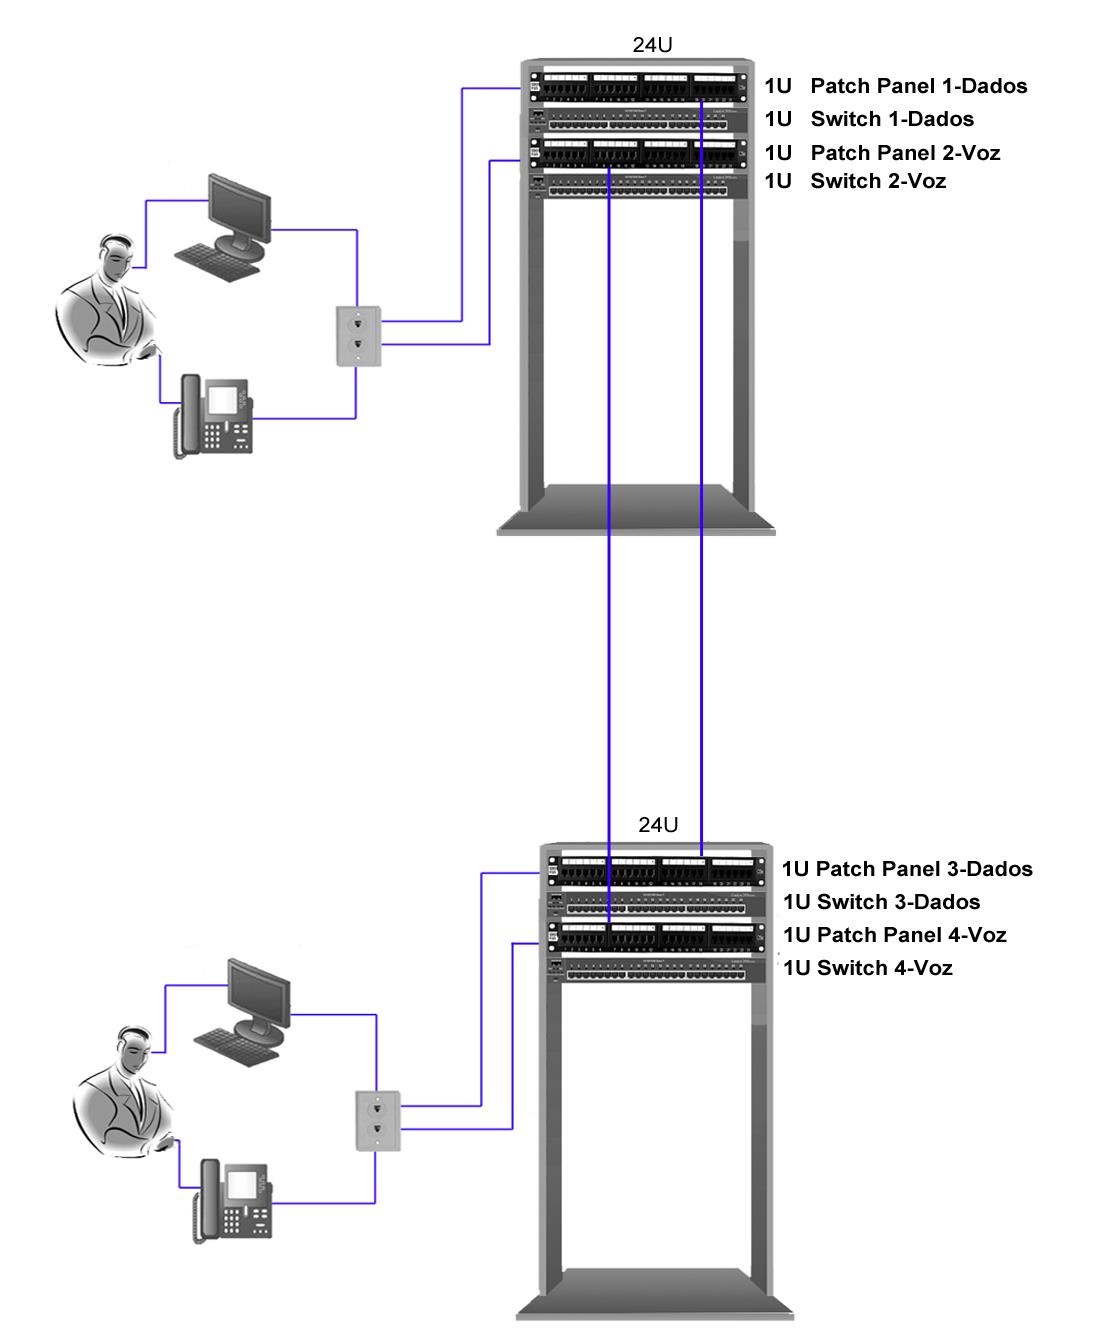
\includegraphics[width=\textwidth]{fig1}
\caption{Exemplo de figura com escala horizontal}
\label{fig1}
\end{figure}


\begin{figure}
	\centering
%%	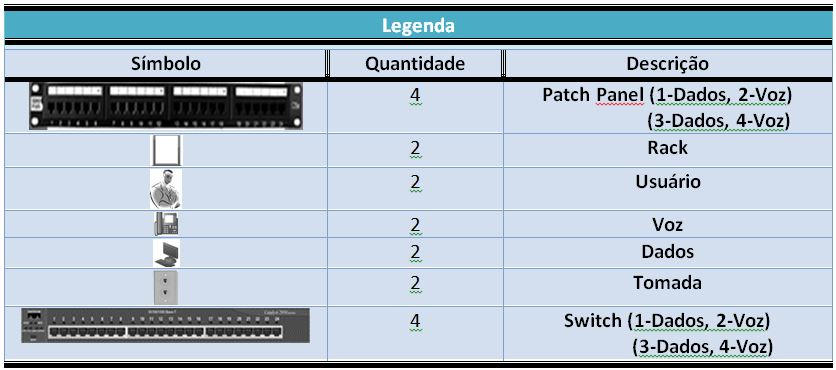
\includegraphics[]{fig2}
	\caption{Exemplo de figura sem escala}
	\label{fig2}
\end{figure}

Você pode rotacionar figuras também. Para isso utilize o parâmetro angle=-90. Repare que a escala da figura foi modificada pelo parametro height. Você também pode utilizar scale

\begin{figure}
	\centering
%%	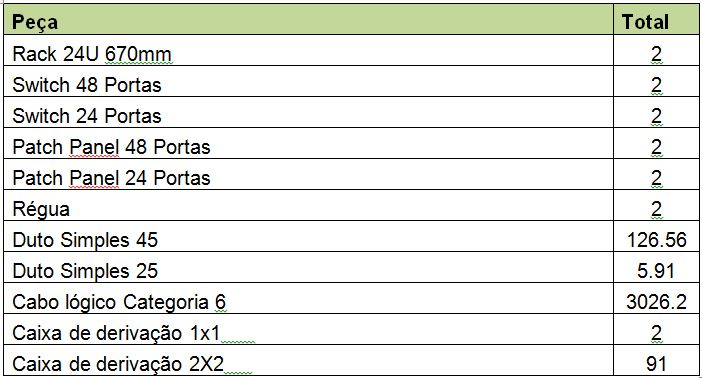
\includegraphics[height=\textwidth,angle=-90]{fig3}
	\caption{Exemplo de figura rotacionada}
	\label{fig3}
\end{figure}


%% ***********************************************************************
%% === ate aqui    =====  ================================================
%% ***********************************************************************
\end{document}